\documentclass[brazil]{../../aerodynamics}

% Metadata
\title{Aerodinâmica Computacional}
\subtitle{Fundamentos, Métodos Numéricos e Aplicações}
\author{Lucas Ribeiro Alves}
\institution{Universidade Federal de Minas Gerais}
\city{Belo Horizonte}
\date{2026}

% References
\addbibresource{../../reference.bib}

\begin{document}
    \frontmatter
    \maketitle
    \tableofcontents
    \chapter{Introdução}
\ChapterTOC

\section{Scope and motivation}
Aerodynamics addresses forces and flows associated with moving bodies and fluids \cite{anderson2017}.

\section{A basic mathematical model}
A simple continuity equation for an incompressible flow is
\begin{equation}
  \nabla \cdot \mathbf{u} = 0.
  \label{eq:continuity}
\end{equation}

\begin{example}
For a uniform two-dimensional flow, $\mathbf{u}=(U_\infty,0)$, the divergence vanishes.
\end{example}

\begin{exercise}
Verify Equation~\eqref{eq:continuity} for the uniform flow above.
\end{exercise}

\begin{remark}
This is a demonstration of the class layout rather than a complete chapter.
\end{remark}

\section{Boundary Layer}

Figure \ref{fig:lam-turb-bl} shows a typical turbulent and laminar boundary layer.

\begin{figure}[h!]
    \centering
    \caption{Comparison between laminar and turbulent boundary layer.}
    % First figure
    \begin{subfigure}[t]{0.48\textwidth}
        \centering
        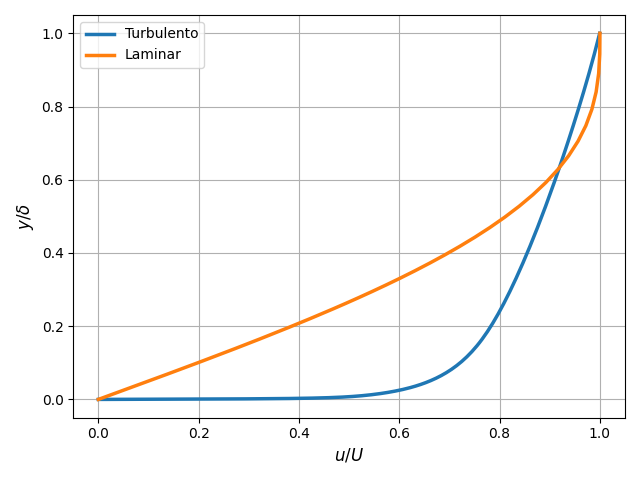
\includegraphics[width=\linewidth]{figures/CHAP-01-FIG-01.png}
        \caption{Boundaer layer.}
        \label{fig:boundary-layer}
    \end{subfigure}
    \hfill
    % Second figure
    \begin{subfigure}[t]{0.48\textwidth}
        \centering
        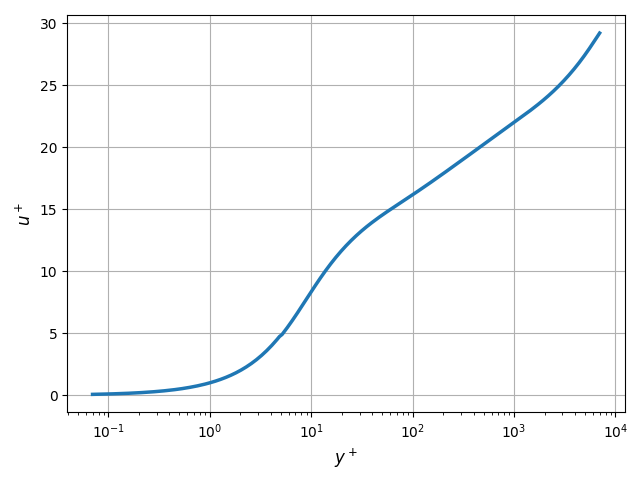
\includegraphics[width=\linewidth]{figures/CHAP-01-FIG-02.png}
        \caption{Law of the wall.}
        \label{fig:law-of-the-wall}
    \end{subfigure}
    \label{fig:lam-turb-bl}
\end{figure}

\ChapterReferences

    \mainmatter
    \part{Método dos Volumes Finitos}
    \chapter{Introdução aos Métodos de Discretização}
\ChapterTOC

\section{Scope and motivation}
Aerodynamics addresses forces and flows associated with moving bodies and fluids \cite{anderson2017}.

\section{A basic mathematical model}
A simple continuity equation for an incompressible flow is
\begin{equation}
  \nabla \cdot \mathbf{u} = 0.
  \label{eq:continuity}
\end{equation}

\begin{example}
For a uniform two-dimensional flow, $\mathbf{u}=(U_\infty,0)$, the divergence vanishes.
\end{example}

\begin{exercise}
Verify Equation~\eqref{eq:continuity} for the uniform flow above.
\end{exercise}

\begin{remark}
This is a demonstration of the class layout rather than a complete chapter.
\end{remark}

\section{Boundary Layer}

Figure \ref{fig:lam-turb-bl} shows a typical turbulent and laminar boundary layer.

\begin{figure}[h!]
    \centering
    \caption{Comparison between laminar and turbulent boundary layer.}
    % First figure
    \begin{subfigure}[t]{0.48\textwidth}
        \centering
        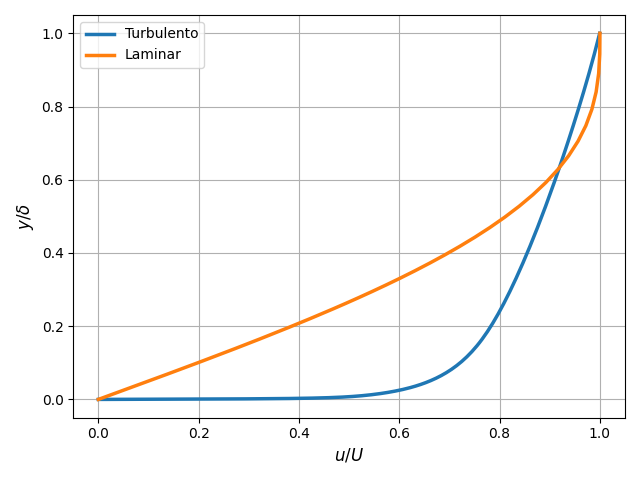
\includegraphics[width=\linewidth]{figures/CHAP-01-FIG-01.png}
        \caption{Boundaer layer.}
        \label{fig:boundary-layer}
    \end{subfigure}
    \hfill
    % Second figure
    \begin{subfigure}[t]{0.48\textwidth}
        \centering
        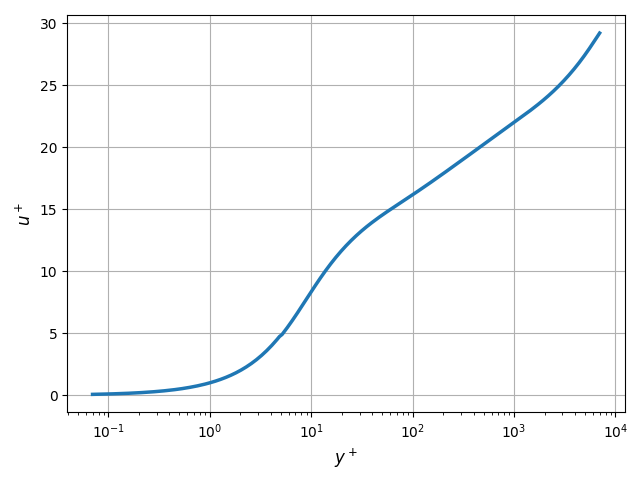
\includegraphics[width=\linewidth]{figures/CHAP-01-FIG-02.png}
        \caption{Law of the wall.}
        \label{fig:law-of-the-wall}
    \end{subfigure}
    \label{fig:lam-turb-bl}
\end{figure}

\ChapterReferences

    \chapter{Fundamentos do Método dos Volumes Finitos}
\ChapterTOC

\section{Potential flow}
An introduction to potential flow and low-speed aerodynamic modeling can be found in \cite{katz2001}.

\section{Governing equations}
For an irrotational velocity field, $\nabla\times\mathbf{u}=\mathbf{0}$.

\ChapterReferences

    \chapter{Geração de Malhas Computacionais}
\ChapterTOC

\section{Potential flow}
An introduction to potential flow and low-speed aerodynamic modeling can be found in \cite{katz2001}.

\section{Governing equations}
For an irrotational velocity field, $\nabla\times\mathbf{u}=\mathbf{0}$.

\ChapterReferences

    \chapter{Métodos de Solução}
\ChapterTOC

\section{Potential flow}
An introduction to potential flow and low-speed aerodynamic modeling can be found in \cite{katz2001}.

\section{Governing equations}
For an irrotational velocity field, $\nabla\times\mathbf{u}=\mathbf{0}$.

\ChapterReferences

    \chapter{Aplicações com OpenFOAM}
\ChapterTOC

\section{Potential flow}
An introduction to potential flow and low-speed aerodynamic modeling can be found in \cite{katz2001}.

\section{Governing equations}
For an irrotational velocity field, $\nabla\times\mathbf{u}=\mathbf{0}$.

\ChapterReferences

    \part{Escoamento Potencial}

    \part{Escoamento Rarefeito}

    \part{Redes Neurais Informadas por Física}
\end{document}
